\section{Case Studies}\label{sec:casestudy}

\subsection{Overview}\label{subsec:cs-overview}

To demonstrate the utility of our modular parsing library, we implemented parsers of the first 18 calculi from book \textit{Types and Programming Languages}. In the book it introduces several calculi from simple to complex, by gradually adding new features to syntax. It is suitable for our case study for mainly two reason. First, the calculi are arguably practical as we want to show our library could be used in real world development. One of the most complex calculi in our case study is System F (with several extensions such as records and variants), which could be the foundation of practical functional programming languages. Second, the evolution of calculi in the book reveals the advantages of modular representation of abstract syntax and modular parsing, which is the key functionality of our library. By decomposing those calculi into smaller components and reusing the common ones, we can obtain considerably code reuse in parsing with little performance penalty, as shown later.

Using the modular parsing techniques discussed before, we extract reusable \textit{components} from syntax of all the calculi. Each component, which may contain several syntactical structures, is a reusable fragment representing a certain feature in the syntax. For example, \lstinline{VarApp} component represents the variable case and application case of expressions. In our case study, each component is represented by a Scala object which has three parts. \lstinline{Alg} is an object algebra interface for the abstract syntax. \lstinline{Print} is an object algebra implements that interface \lstinline{Alg}, for the pretty printing operation. It is not necessary for parsing, but we include it here for demonstration. \lstinline{Parser} is the modular parser for this piece of syntax.

\begin{lstlisting}
object VarApp {
  trait Alg[E] {
    def TmVar(x: String): E
    def TmApp(e1: E, e2: E): E
  }
  trait Print extends Alg[String] {
    def TmVar(x: String) = x
    def TmApp(e1: String, e2: String) = "[" + e1 + " " + e2 + "]"
  }
  trait Parser[E, F <: {val pE : PackratParser[E]}] {
    lexical.delimiters += ("(", ")")
    val pVarAppE: Alg[E] => (=> F) => PackratParser[E] = alg => l => {
      val e = l.pE
      ident ^^ alg.TmVar |||
      e ~ e ^^ { case e1 ~ e2 => alg.TmApp(e1, e2) } |||
      "(" ~> e <~ ")"
    }
  }
}
\end{lstlisting}

We use some naming conventions in our code, \lstinline{E} represents expressions, \lstinline{T} represents types and \lstinline{K} represents kinds. In this component \lstinline{VarApp} we only have expressions. The \lstinline{Alg} and \lstinline{Print} are standard object algebra operations, thus we will focus on the modular parser \lstinline{Parser}. Each parser carries lexical information and parsing functions. The lexical information includes reserved words, delimiters, etc. Parsing functions are similar with we described before, except that we use record types under some subtyping constraints here for the explicit self-reference. The record type contains a parser for expressions \lstinline{pE}, a parser for types \lstinline{pT} and a parser for kinds \lstinline{pK}, if the corresponding one is needed when parsing the syntax of this component. Here the type of self-reference, namely \lstinline{F}, is only required to have a parser of expressions \lstinline{pE}. Then we can build the parsing function \lstinline{pVarAppE}, the suffix \lstinline{E} also denotes that it will parse an expression.

Each calculus could be composed directly from components and other calculi, if it has those common structures in the syntax. For example, the calculus \lstinline{Untyped}, representing the famous untyped lambda calculus, can be constructed from components \lstinline{VarApp} and untyped lambda abstraction \lstinline{UntypedAbs}.

\begin{lstlisting}
object UntypedAbs {
  trait Alg[E] {
    def TmAbs(x: String, e: E): E
  }
  trait Print extends Alg[String] {
    def TmAbs(x: String, e: String) = "\\" + x + "." + e
  }
  trait Parser[E, F <: {val pE : PackratParser[E]}] {
    val pUntypedAbsE: Alg[E] => (=> F) => PackratParser[E] = {...}
  }
}

object Untyped {
  trait Alg[E] extends UntypedAbs.Alg[E] with VarApp.Alg[E]
  trait Print extends Alg[String] with UntypedAbs.Print with VarApp.Print
  trait Parser[E, L <: {val pE : PackratParser[E]}] extends UntypedAbs.Parser[E, L] with VarApp.Parser[E, L] {
    val pUntypedE = pUntypedAbsE | pVarAppE
  }
}
\end{lstlisting}

When composing the calculus from components, all the fields can be easily combined by Scala’s \lstinline{extends...with} keywords as shown in the code. For \lstinline{Parser}, the subtyping constraint for the explicit self-reference should satisfy all the requirement of the parsers it extends from. \huang{Talk about | here?}

Finally, we have demo code for every calculus. The parsing result is a string because we provide the pretty printing algebra to the parser, and it can be changed as long as the concrete algebra is available. In this case study we only have pretty printing as the operation, since it is enough for demonstration.

\begin{lstlisting}
object TestUntyped {
    to be polished
}
\end{lstlisting}

In the next section we will show more examples and talk further about how we extend and compose these components and calculi.

\subsection{Extensibility}\label{subsec:cs-extensibility}

\begin{figure}
    \centering
    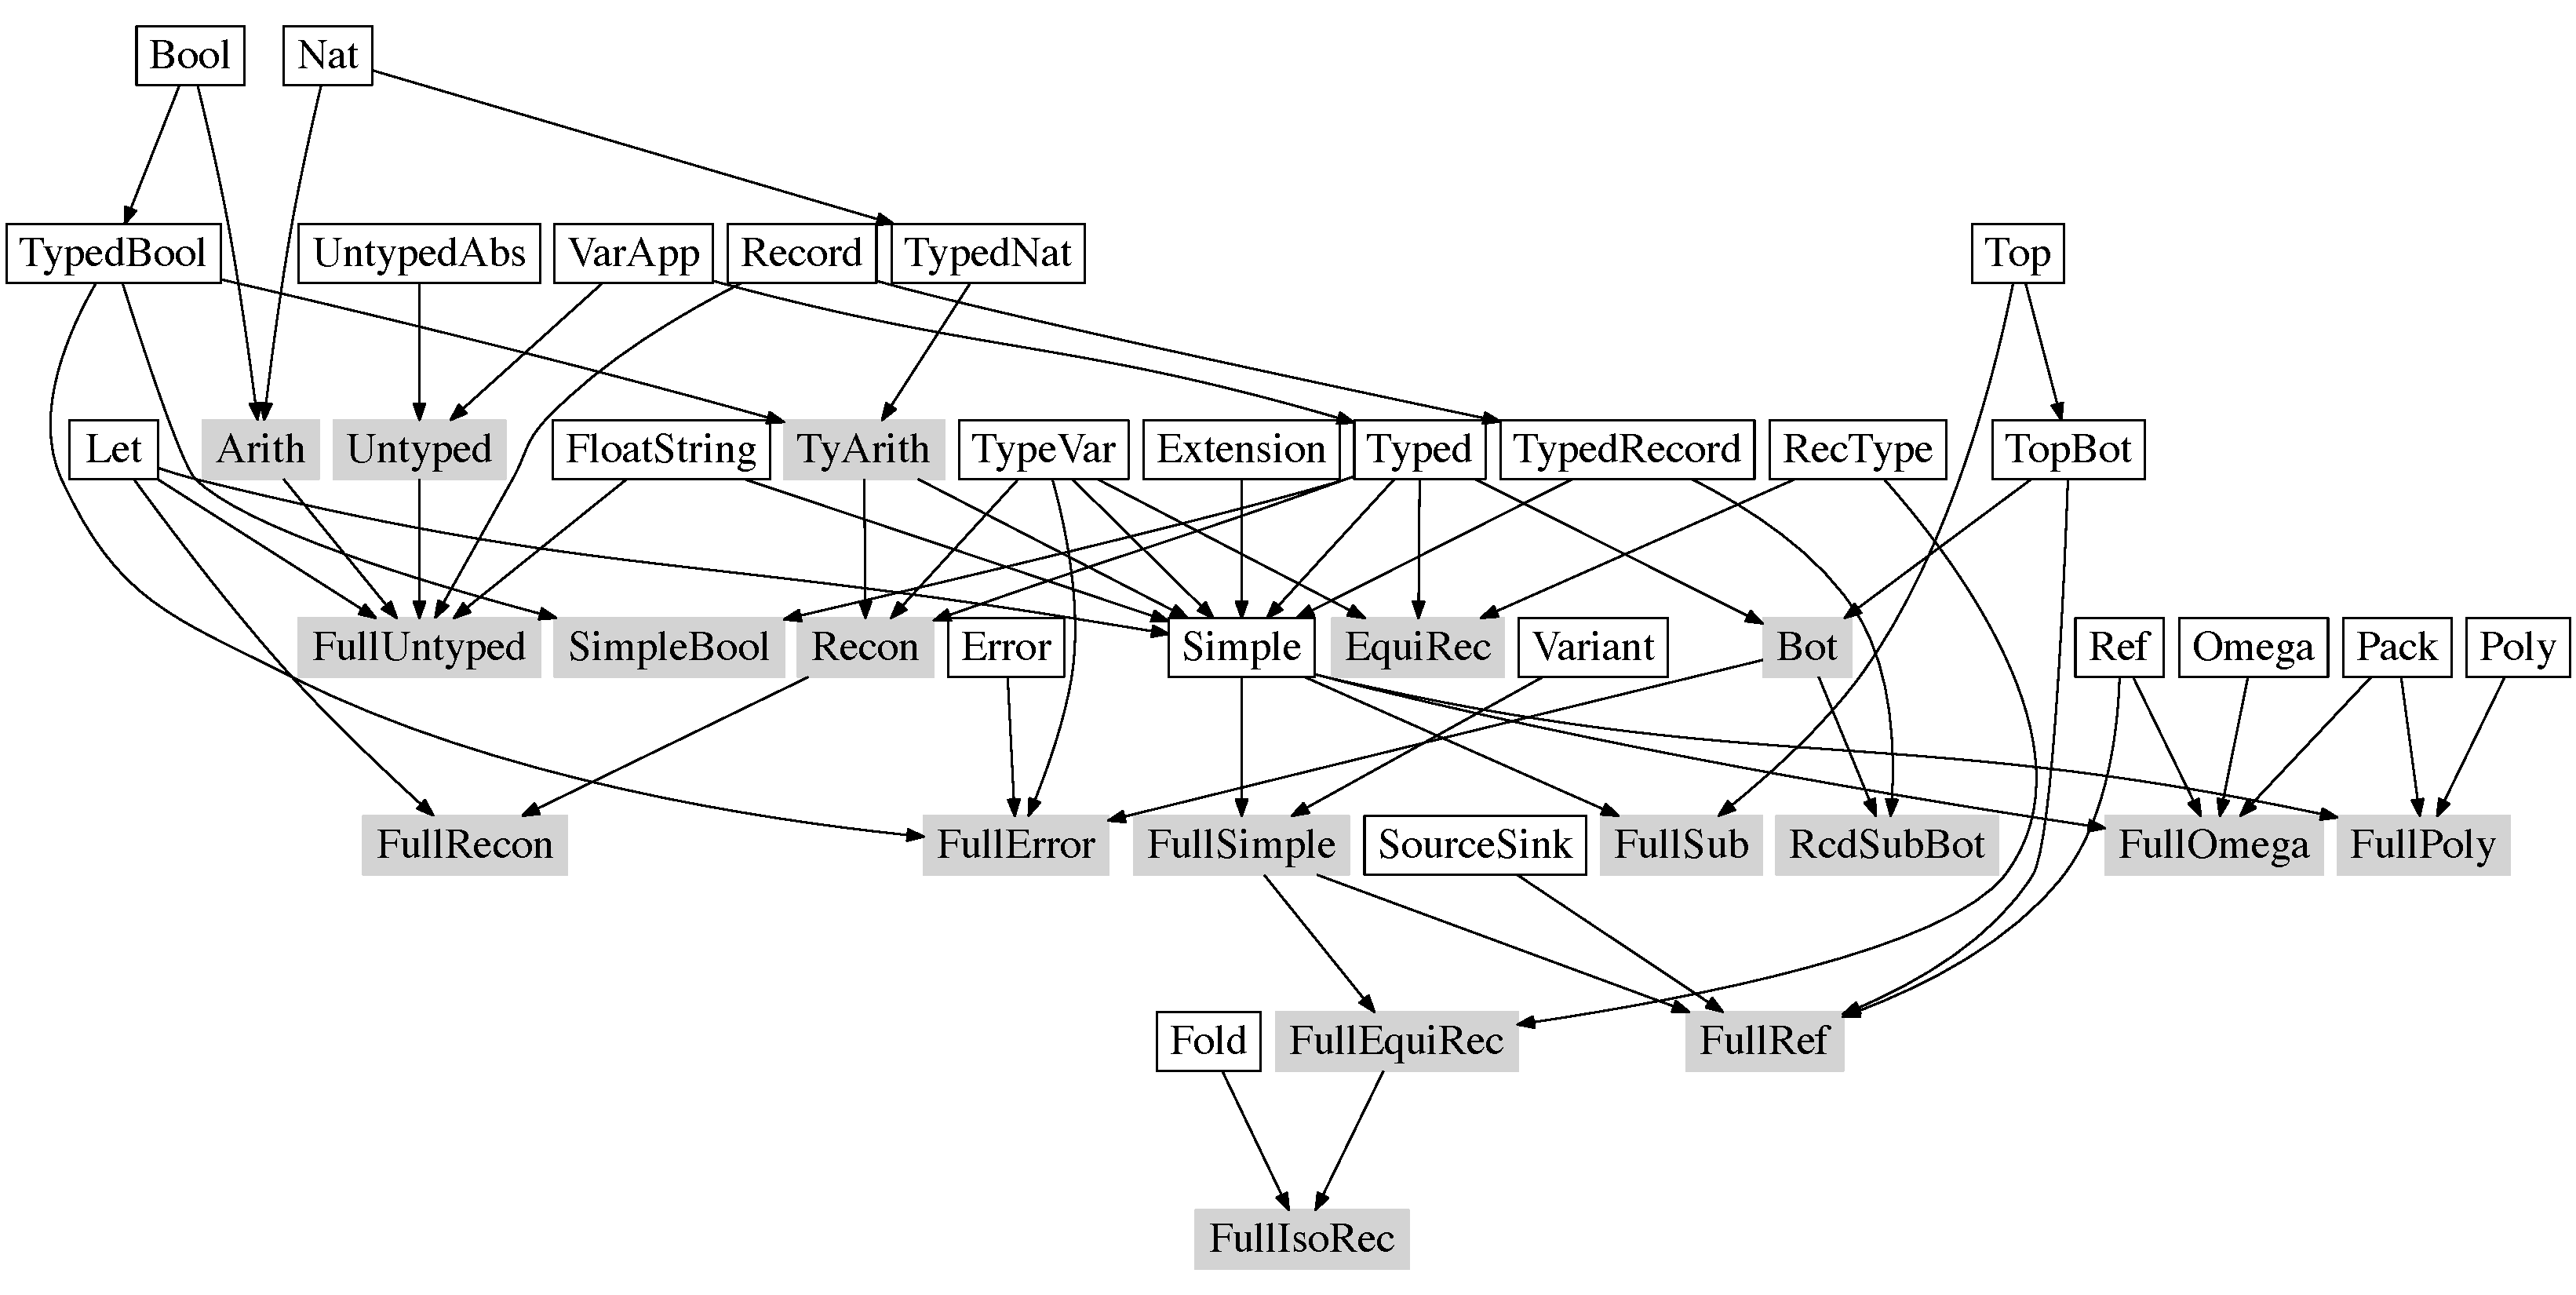
\includegraphics[width=\textwidth]{resources/depGraph.pdf}
    \caption{Dependency graph of all calculi and components}
    \label{fig:dependency}
\end{figure}

As mentioned before, we decompose all the calculi into reusable components for modularity. Figure \ref{fig:dependency} shows the dependency of all the components and calculi in our case study. Gray boxes are calculi and white boxes are components. An arrow starting from box A to box B denotes that B includes and thus reuses A.

As shown in the graph, some components such as \lstinline{VarApp} are created from scratch, while others such as \lstinline{Typed} are extended from existing components. The \lstinline{Typed} component extends from \lstinline{VarApp} and has two more syntactical structures which are typed lambda abstraction and function type (arrow type). It is the core of many calculi in this case study, and we use it here as an example for demonstrating the extensibility of components.

\begin{lstlisting}
object Typed {
  trait Alg[E, T] extends VarApp.Alg[E] {
    def TmAbs(x: String, t: T, e: E): E
    def TyArr(t1: T, t2: T): T
  }
  trait Print extends Alg[String, String] with VarApp.Print {
    def TmAbs(x: String, t: String, e: String) = "\\(" + x + ":" + t + ")." + e
    def TyArr(t1: String, t2: String) = t1 + "->" + t2
  }
  trait Parser[E, T, F <: {val pE : PackratParser[E]; val pT : PackratParser[T]}] extends VarApp.Parser[E, F] {
    ...
    private val pAbsE: Alg[E, T] => (=> F) => PackratParser[E] = {...}
    val pTypedE: Alg[E, T] => (=> F) => PackratParser[E] = pVarAppE | pAbsE
    val pTypedT: Alg[E, T] => (=> F) => PackratParser[T] = alg => l => {
      val t = l.pT
      t ~ ("->" ~> t) ^^ { case t1 ~ t2 => alg.TyArr(t1, t2) } ||| "(" ~> t <~ ")"
    }
  }
}
\end{lstlisting}

Except building a component by extending an existing one, here we have another extension which is adding a new sort of syntax. It has been discussed in section \ref{subsec:openrecursion}. In this example, originally \lstinline{VarApp} has only one sort of syntax which is expressions, and then \lstinline{Typed} introduces types to the syntax. We add an extra type parameter \lstinline{T} for it, so that it is able to be distinguished. The \lstinline{Parser} also requires the self-reference to have a field \lstinline{pT} for parsing types, which is represented by the subtyping constraint. With this support, the \lstinline{pTypedT} function parses arrow types using \lstinline{pT}. Another point worth mentioning is that we use a private local function \lstinline{pAbsE} here for parsing the typed lambda abstraction case, and we can directly combine it with the inherited \lstinline{pVarApp} to obtain our parsing function of expressions.

Since calculi and components have the similar signature, each calculus can also be extended and reused directly. Our last example shows how to build calculus \lstinline{FullRef} from extending \lstinline{FullSimple}, another calculus.

\begin{lstlisting}
object FullRef {
  trait Alg[E, T] extends FullSimple.Alg[E, T] with TopBot.Alg[T] with Ref.Alg[E, T]
  trait Print extends Alg[String, String] with FullSimple.Print with TopBot.Print with Ref.Print
  trait Parser[E, T, L <: {val pE : PackratParser[E]; val pT : PackratParser[T]}] extends FullSimple.Parser[E, T, L] with TopBot.Parser[T, L] with Ref.Parser[E, T, L] {
    val pFullRefE = pFullSimpleE | pRefE
    val pFullRefT = pFullSimpleT | pRefT | pTopBotT
  }
}
\end{lstlisting}

Using our modular parsing library, dividing the syntax into small pieces and bind them with corresponding parsers to form reusable language component is convenient. From the dependency graph we know that the common components such as \lstinline{VarApp} are reused in lots of calculi. Such reuse could shorten the code considerably. We will show this advantage and exam the possible performance penalty in a quantitative way in the next section.

\subsection{Comparison}\label{subsec:cs-comparison}

We compared our implementation of the parsers with an implementation we found online, written by author Ilya Klyuchnikov. Ilya's implementation is very suitable for comparison, because it is also written in Scala using the same parser combinator library. Furthermore, it includes parsers of all the 18 calculi we have, but written in a non-modular way. Thus it is not able to reuse existing code of parsing common syntactical features.

Because Ilya's implementation has extra code such as semantics of those calculi, we removed all irrelevant code and only keep abstract syntax definition, parser and pretty printer for each calculus, to ensure a fair comparison.

The comparison is made from two aspects. First, we want to show that using our modular parsing library, the code can be reused in a significant way. For this propose, we measured source lines of code (SLOC) of the two implementations. All blank lines and comment lines are excluded, and we formatted the code of both implementations so that the length of each line does not exceed 120 characters. Second, users may concern the performance penalty caused by modularity. Thus we compared the execution time, as a major measurement of performance, between the two implementations. We prepared test files containing valid expressions in each calculus, then we used the corresponding parser to parse the file and the pretty printer to print the result. The execution time excluding reading input file was calculated.

\begin{table}
    \centering
    \begin{tabular}{|l|r|r|r|r|r|r|}
      \hline
        \multirow{2}{*}{\bfseries Calculus Name} & \multicolumn{3}{ c| }{\bfseries SLOC} & \multicolumn{3}{ c| }{\bfseries Time (ms)} \\ \cline{2-7}
        \multicolumn{1}{|c|}{} & \bfseries Ilya's & \bfseries Ours & \bfseries (+/-)\% & \bfseries Ilya's & \bfseries Ours & \bfseries (+/-)\% \\
      \hline
      \begin{tabular}{|c|c|c|}
  \hline
  t1 & t2 & t3 \\
  y1 & val1 & val4 \\
  y2 & val2 & val3 \\
  \hline
\end{tabular}

      \hline
    \end{tabular}
    \caption{Comparison of SLOC and execution time}
    \label{tab:comparison}
\end{table}

Table \ref{tab:comparison} shows data of the comparison. The overall result of SLOC comparison is that 66.3\% of code is reduced using our library. That is because the code of some common syntax structures such as variable, lambda abstraction, etc., is reused several times in the whole project. We can see that the first two calculi \lstinline{Arith} and \lstinline{Untyped} we do worse than Ilya's implementation, because in such two cases we do not reuse any existing components. But in each of the following 16 calculi, we can compose our syntax definition, parser and pretty printer from extending reusable components, resulting considerably code reduction.

For the execution time comparison, we built a generator to randomly generate valid expressions according to the syntax of each calculus. Each test file corresponds with one calculus and it consists of 500 expressions randomly generated. The size of test files varies from 20KB to 100KB. After testing both implementation, we found that our version is about \huang{60\%} slower. Part of the reason is that our library requires more intermediate function calls, and the object algebra and self-reference needed to be passed as arguments every time. However, another important reason is that, because of the modular setting, we use a different alternative combinator which will try both branches and match the longest one. \huang{ref to somewhere before?} In contrast Ilya uses the ordinary alternative combinator which tries the second branch only if the first one fails. Although this difference slows our version, we want to mention that because of the memorization of Packrat parsers, we are just constant times slower, the big-O complexity is still the same.


